\documentclass[a4paper]{article}

\input ../header
\usepackage[np]{numprint}
\usepackage{xcolor}
\usepackage{booktabs}
\usepackage{gensymb}

\setlength{\multicolsep}{2pt}

\begin{document}

\title{Activités -- Mobiliser les acquis sur les fonctions}

\pagestyle{empty}

\date{}
\author{}

\maketitle{}
\thispagestyle{empty}

\exo Pour chacune des situations suivantes, exprimer les quantités demandées \og{}en fonction de\fg{}la quantité indiquée.

\begin{enumerate}
  \item Un vase a la forme d'un pavé droit de base carrée de côté $c$ cm. On remplit d'eau ce vase jusqu'à une hauteur de $15$ cm. Exprimer, en fonction de $c$, le volume d'eau (en cm$^3$) contenu dans ce vase.
  \item Un cinéma propose à ses clients une carte annuelle à $25$ \euro{} qui permet ensuite de payer $4$ \euro{} par séance au cours de l'année. Exprimer le coût total (en euros) en fonction du nombre $N$ de séances achetées dans l'année pour un client détenant cette carte.
  \item Pour clôturer une parcelle de terrain, on utilise une clôture d'une longueur de $100$ mètres. On note $x$ la largeur de cet enclos. Exprimer en fonction de $x$ l'aire $\mathcal{A}(x)$ de la parcelle.
\end{enumerate}

\bigskip

\exo Enzo a besoin d'un seau d'eau pour aller pêcher. En une minute, il a rempli le seau d'une contenance de $3$ L. Quand il commence à le remplir, le seau est vide. Une minute après, le seau est plein et il n'a jamais renversé d'eau. Parmi les graphiques ci-dessous, lesquels ne peuvent pas représenter le volume d'eau (en L) dans le seau en fonction du temps (en s) ?

\begin{center}
  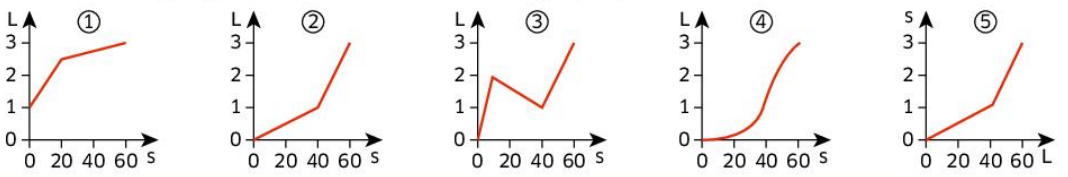
\includegraphics[width=16cm]{7_1_mobiliser_les_acquis_sur_les_fonctions_seau.png}
\end{center}

\bigskip

\exo On considère le programme de calcul ci-dessous qui définit une fonction $g$ :

\begin{center}
  \fbox{
    \begin{minipage}{5cm}
      \begin{itemize}
	\item Choisir un nombre
	\item Ajouter $5$
	\item Prendre le carré de la somme obtenue
      \end{itemize}
    \end{minipage}
  }
\end{center}

\begin{enumerate}
  \item 
    \begin{enumerate}
      \item Quel résultat obtient-on quand on choisit le nombre $3$ ?
      \item Quelle est l'image de $-7$ par $g$ ?
    \end{enumerate}
  \item Peut-on obtenir $-25$ ?
  \item Parmi les fonctions suivantes, quelle est la fonction $g$ ?
    \begin{multicols}{4}
      \begin{enumerate}
	\item $x\mapsto x^2+25$
	\item $x\mapsto x^2+5$
	\item $x\mapsto (x+5)^2$
	\item $x\mapsto 2(x+5)$
      \end{enumerate}
    \end{multicols}
\end{enumerate}

\bigskip

\exo Soit $h$ la fonction définie sur $\mathbb{R}$ par $h(x)=2x^2+4x-5$.
\begin{enumerate}
  \item Calculer l'image de $-1$ par $h$.
  \item Calculer $h(2)$.
  \item Trouver les antécédents de $-5$ par $h$.
\end{enumerate}

\pagebreak

\exo Un avion de ligne effectue un vol de Toulouse vers Paris. Ses capteurs de température extérieure ont fourni des données tout au long du vol. La situation est modélisée par une fonction $f$ représentée ci-dessous :

\begin{center}
  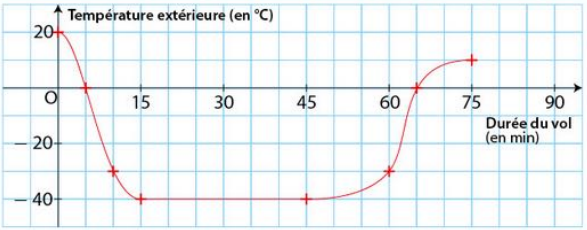
\includegraphics[width=13cm]{7_1_mobiliser_les_acquis_sur_les_fonctions_temperature_exterieure.png}
\end{center}

\begin{enumerate}
  \item Combien de temps le vol a-t-il duré ?
  \item Quel est l'ensemble de définition de la fonction $f$ ?
  \item Préciser l'image de $15$ par $f$, puis donner un antécédent de $-30$ par $f$.
  \item Donner un nombre n'ayant pas d'antécédent par $f$.
  \item Quelle température faisait-il cet après-midi là :
    \begin{enumerate}
      \item à Paris ?
      \item à Toulouse ?
    \end{enumerate}
\end{enumerate}


\end{document}
